%% Hanford investigations

%% TCS schematic for LIGO Hanford for O3
%% TCS pre-loading
 %% Current methodology for tuning TCS
  %% Detail Hanford's methods
 %% Increasing RH tuning speed


As shown in Chapter 1,  increasing input power directly relates to an interferometer's sensitivity to detecting gravitational waves. This comes with a few implications, but one in particular is the necessity for thermal compensation. As the interferometer increases input power, you directly couple more light into the Fabry-P\'{e}rot cavity arms. The optics, even with super low absorption ($\approx$ 400 ppb) still induce thermo-optic effects with the projected circulating arm power of 200 kW. A symptom of this is mode mismatching throughout the interferometer, a problem that contributes to loss of optical power at the anti-symmetric port which can reduce sensitivity two-fold: loss of power to your readout and reduced efficacy of implementing quantum squeezing.

\subsection{TCS preloading for O3}
Reference to TVO's thesis for preloading settings based on his model\cite{tvo}

\subsection{Point absorbers}
Coupling into control signals (ASC and LSC)
\begin{itemize}
\item Loss of interferometer control
\item Reported in "TCS comissioning for O3" @ LVK, I reference a Craig elog where he reports loss of sideband power after thermalization (particularly POP LF, REFL LF, POP 18, POP 45)
\item A. Brooks explains in \cite{brooks2021}
\end{itemize}


\subsection{RH input conditioning}
Some notes about the analytical calculations of RH (There is a paper on this).
Notes as to why this 12 hour time constant is not optimal for thermal compensation.
\section{Optimizing thermo-optic response}

\begin{figure}[H]
 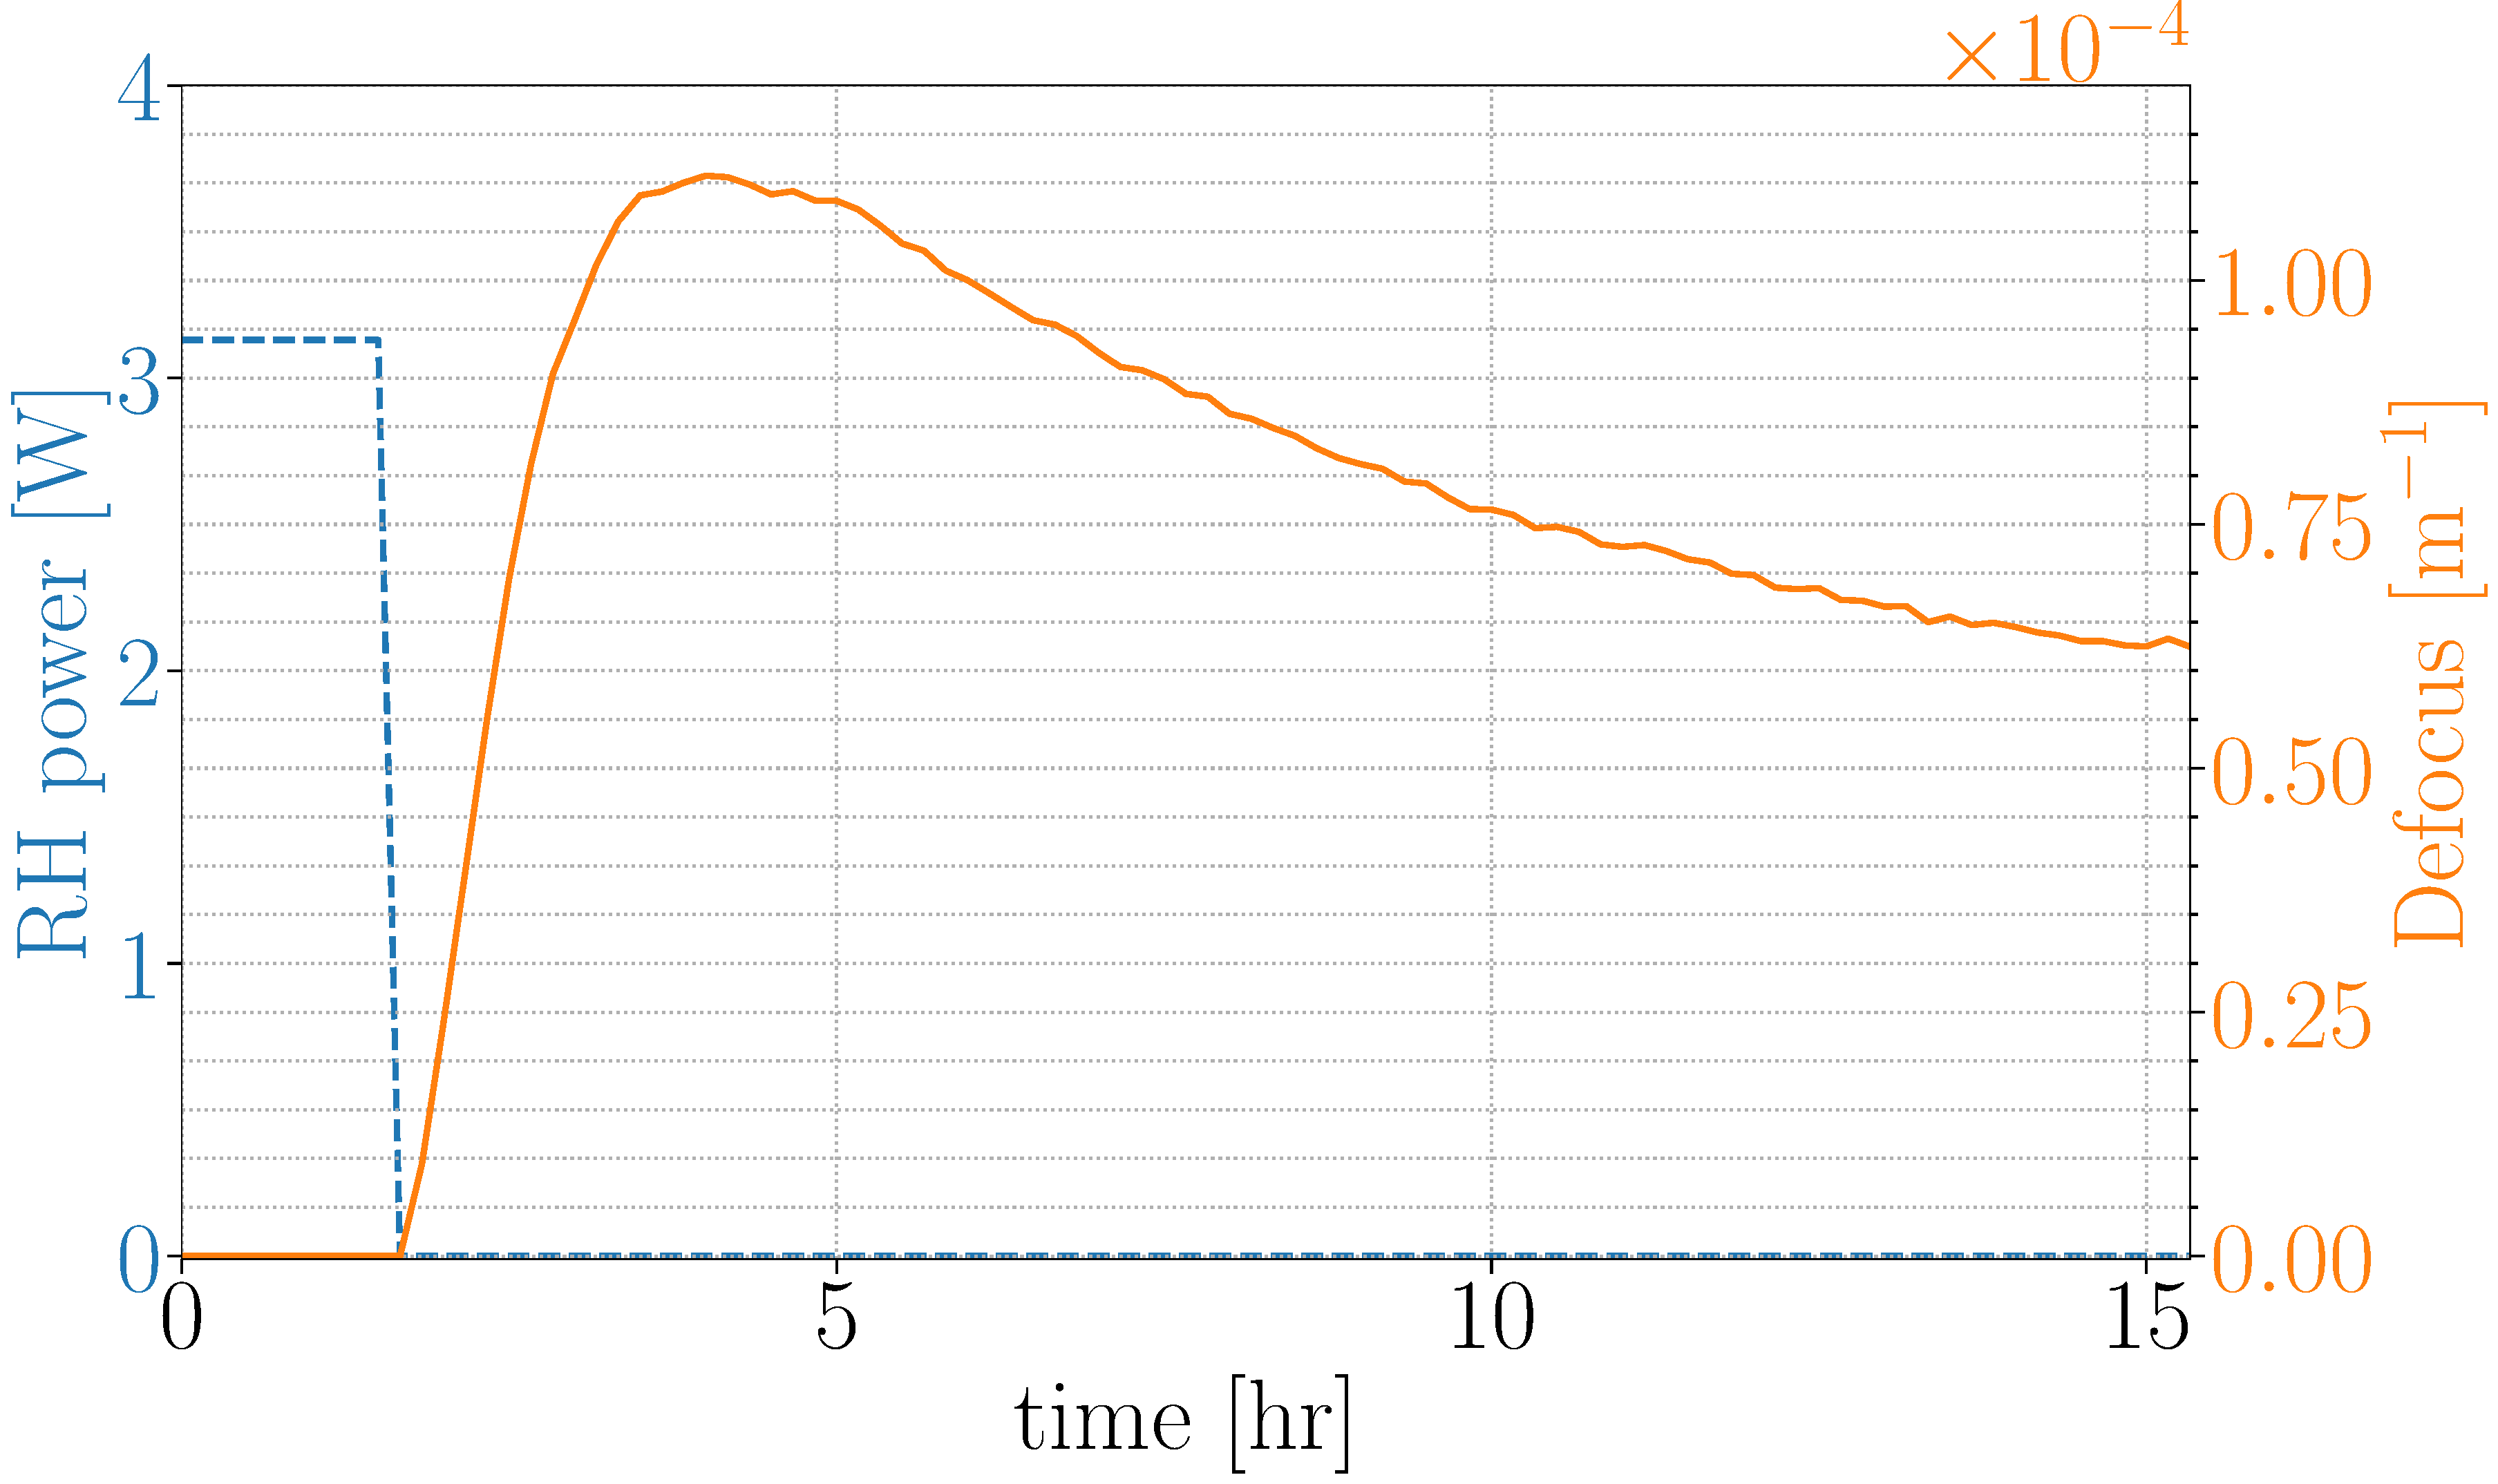
\includegraphics[width=\textwidth]{TCS/IRHF/Meas_response}
 \caption{ITMY thermo-optic response to a 3.13 Watt power reduction to ring heaters. It's after $\approx$ 12 hours after the change was made do you start to see a small enough $\frac{\mathrm{d} \alpha_\mathrm{sp}}{\mathrm{dt}}$ when you can assume a steady thermal lens.}
 \label{fig:meas}
\end{figure}


\begin{figure}[H]
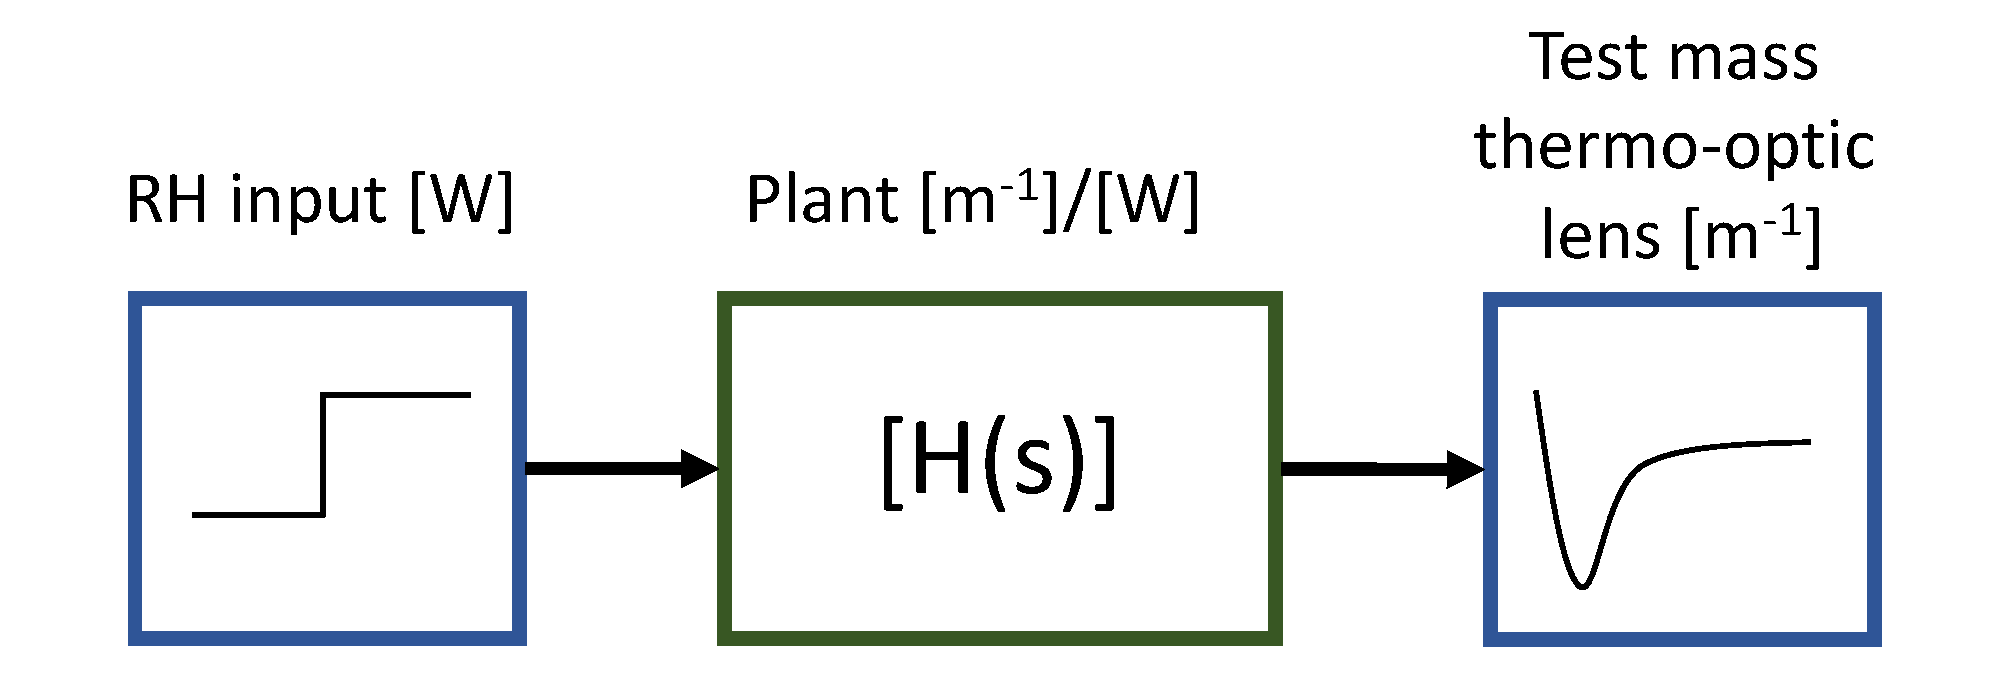
\includegraphics[page=1,width=\textwidth]{TCS/IRHF/RH_input_filter_figures.pdf}
\caption{A pictograph showing how the plant transforms the signal. The example of this can be seen in Fig [\ref{fig:meas}]}
\label{fig:justplant}
\end{figure}

\begin{figure}[H]
\includegraphics[page=2,width=\textwidth]{TCS/IRHF/RH_input_filter_figures.pdf}
\caption{A pictograph showing the system with real time digital filtering for an improved thermo-optic response. The RH input filter is created by inverting the plant filter combine with a low pass and added poles to the zpk model to ensure stability.}
\label{fig:plantwfilt}
\end{figure}

\begin{figure}[H]
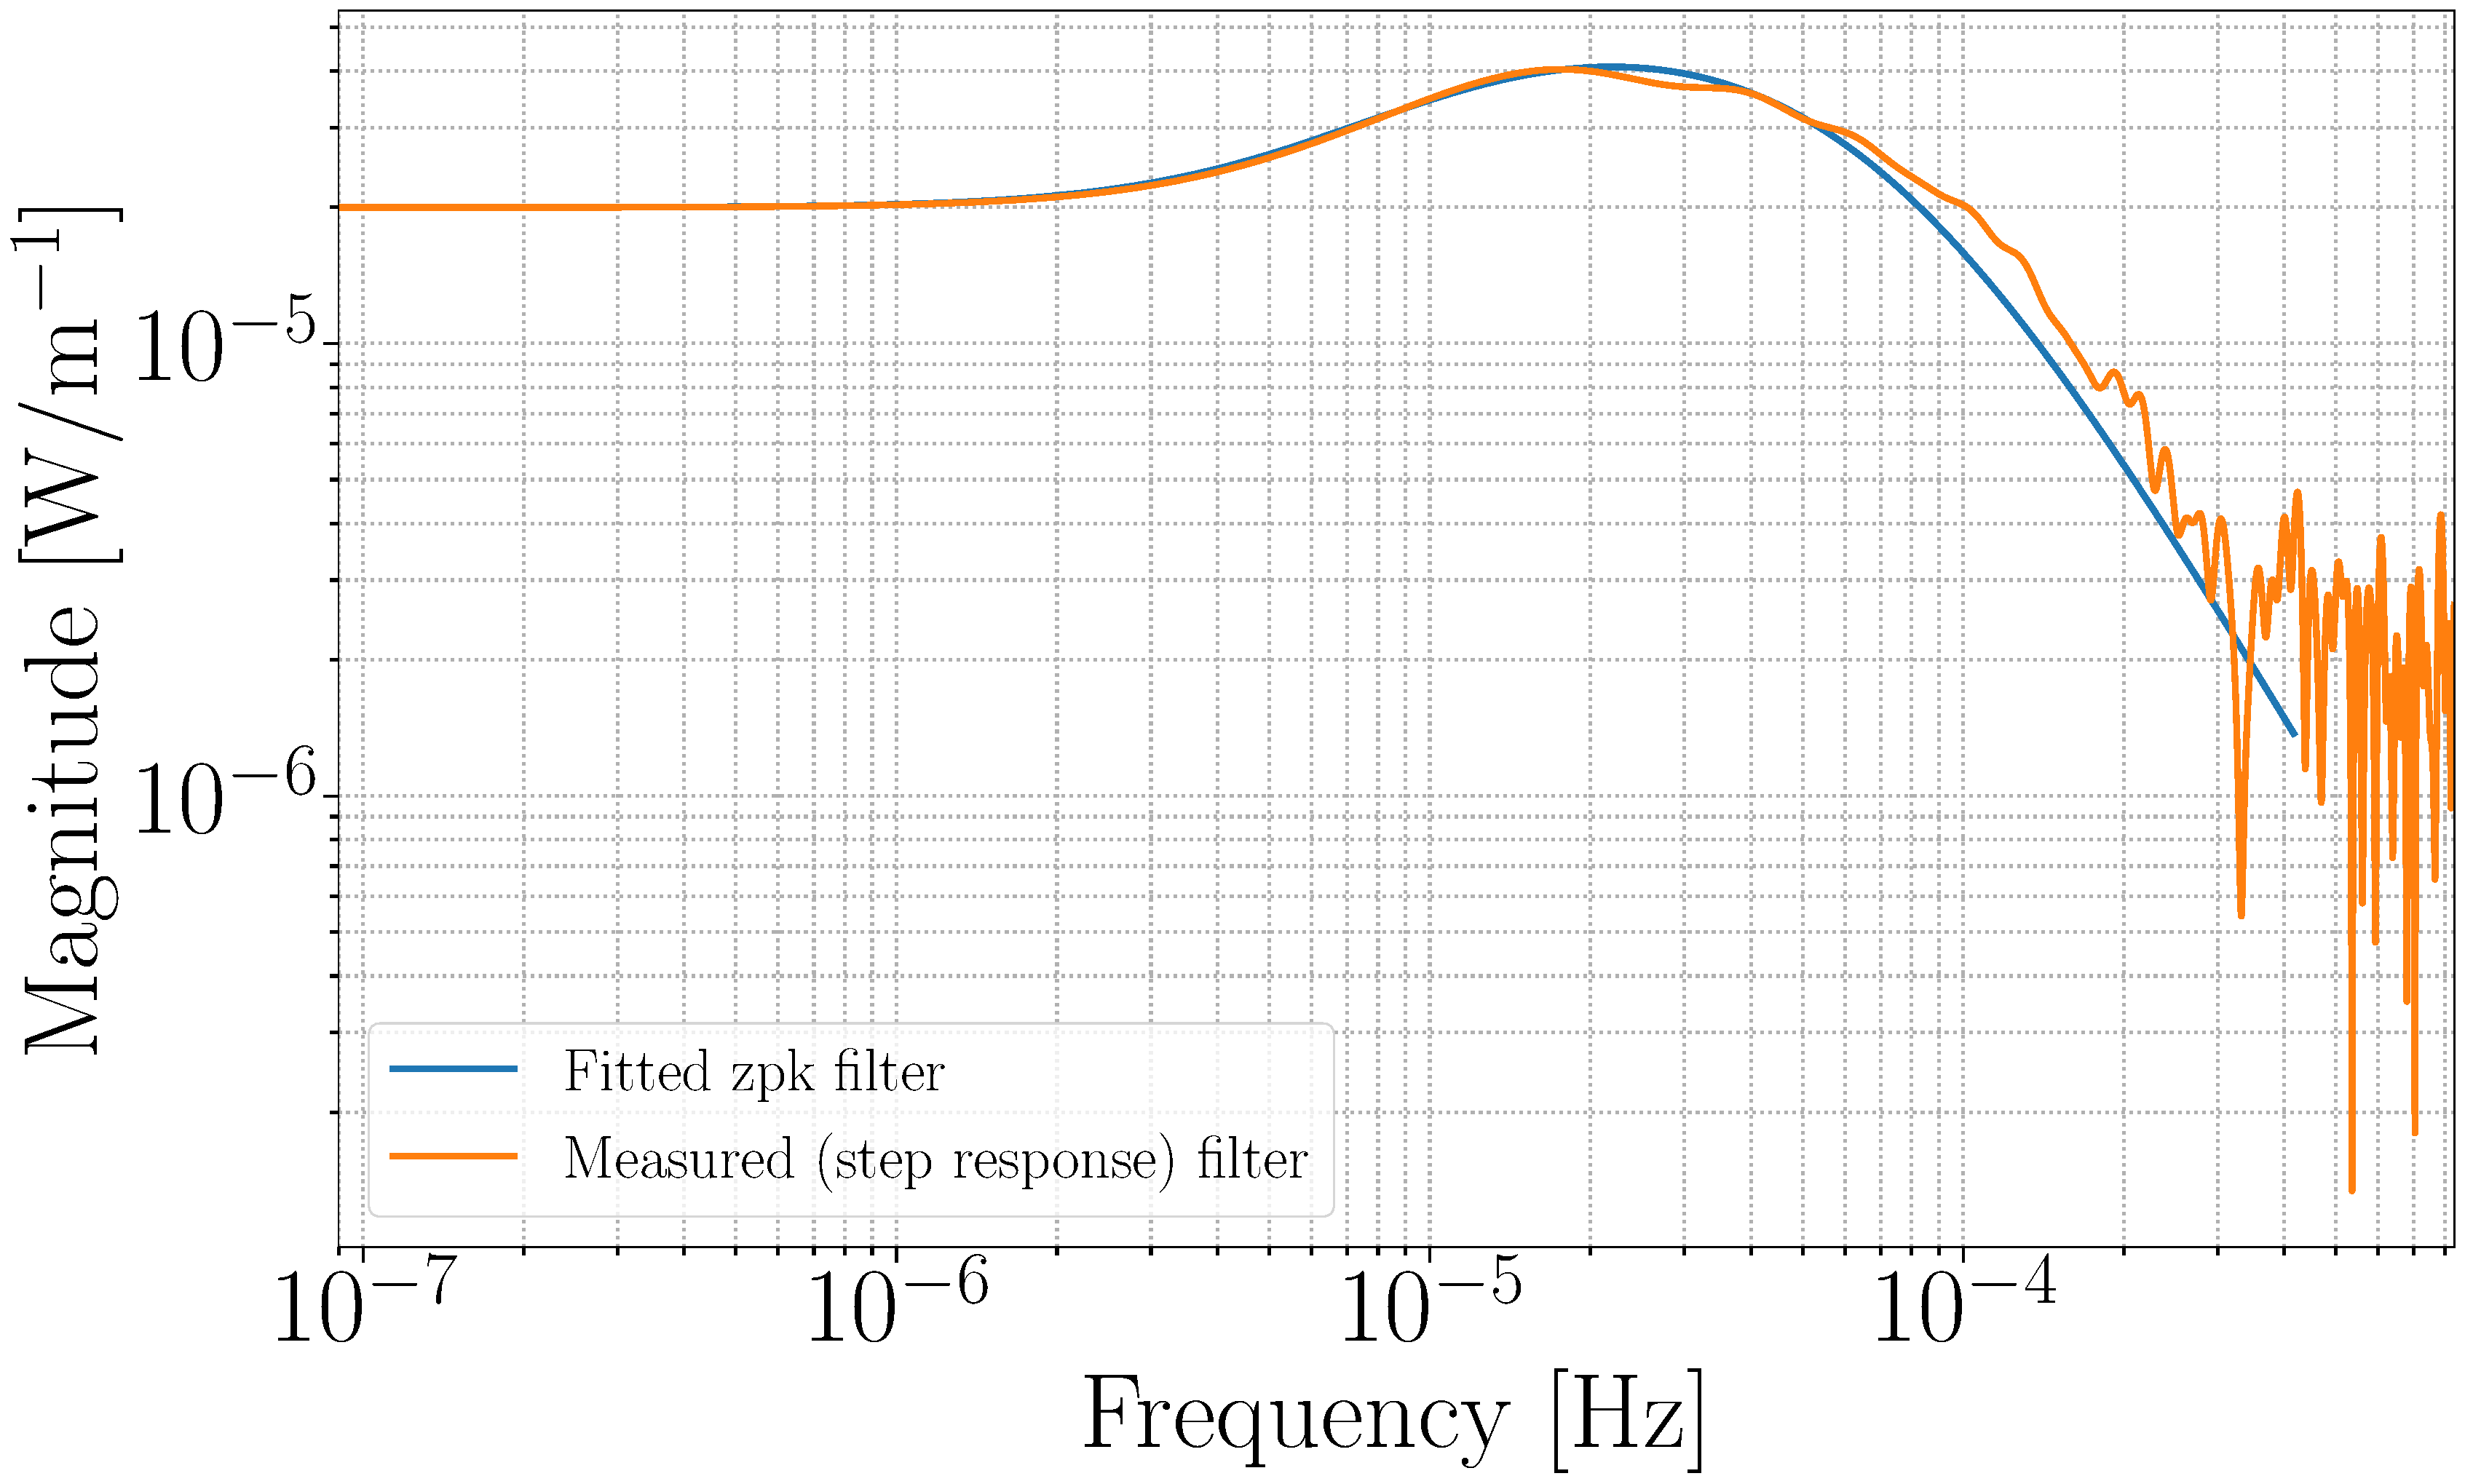
\includegraphics[width=\textwidth]{TCS/IRHF/RH_plant_filter_fit}
\caption{Showing the PSD of the RH response (normalized by the input RH power) over a an $\approx$ 12.5 hour period. The zpk model of the fitted filter (H(s)) is $9.2545e-12 \frac{(s+3.14210e-5)}{(s+8.168e-5)(s+0.0003142)(s+0.0005969)}$}
\label{fig:plant_v_fit}
\end{figure}

\section{Dynamic Thermal compensation}
\begin{figure}[H]
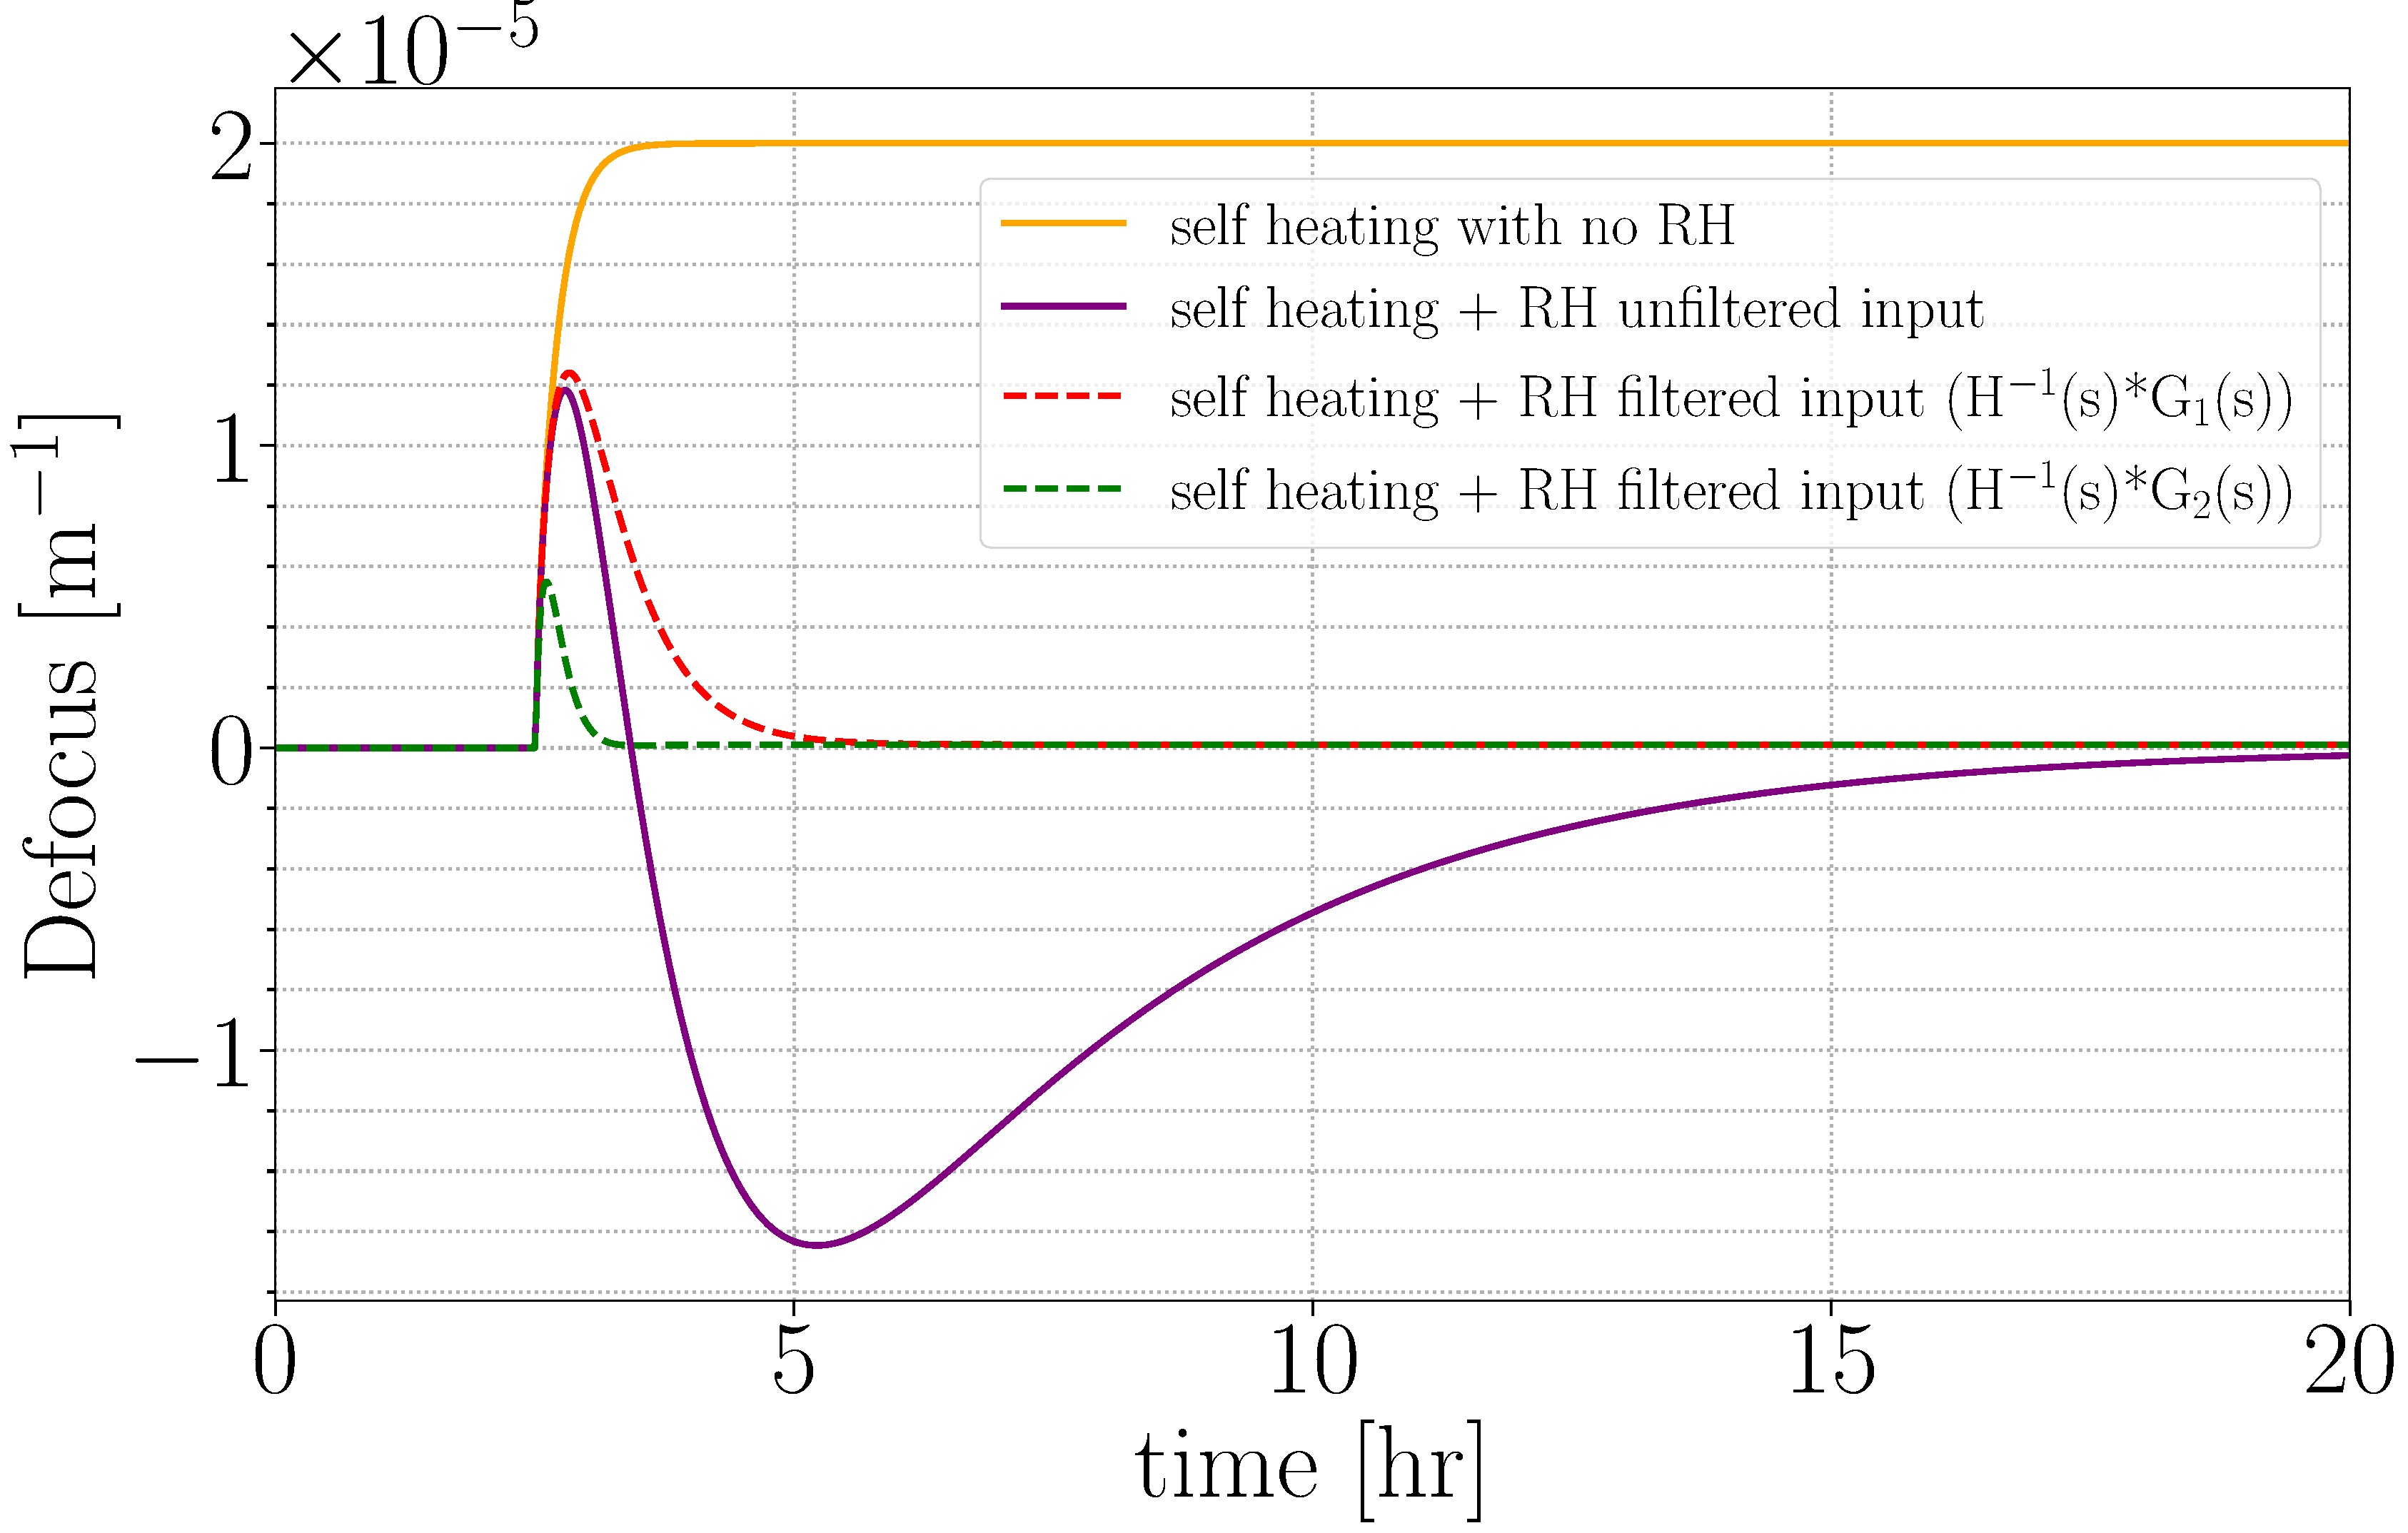
\includegraphics[width=\textwidth]{TCS/IRHF/IRHF_compare_w_self}
\caption{Comparison of the natural RH response and the response to the conditioned input. The above plot is simulated in Matlab by passing the RH input time series (top plot) through the $[H(s)]^{-1*}$ and $H(s)$ to acquire with the result lensing behavior on the bottom plot.}
\label{fig:dynam_comparison}
\end{figure}
\newpage

\textbf{Analytical expression of self heating from beam} \cite{hello_vinet}

\section{Limitations}
